\documentclass[a4paper,12pt]{article}

\usepackage[utf8]{inputenc}
\usepackage[T1]{fontenc}
\usepackage[french]{babel}
\usepackage{geometry}
\usepackage{graphicx}
\usepackage{url}
\usepackage{hyperref}
\usepackage{natbib}
\usepackage{authblk}
\usepackage{color}

\usepackage{amsmath,amsfonts,amssymb,amsthm,mathrsfs}
\usepackage{tabularx}
\usepackage{array}
\usepackage{makecell}
\usepackage{ragged2e} % Pour la commande \RaggedRight
 
\geometry{
    left=2.5cm,
    right=2.5cm,
    top=2.5cm,
    bottom=2.5cm
}


\title{Qui influence la décision politique en France?}
\author[1]{Rapha\"el Lachièze-Rey}



\begin{document}

\maketitle

\begin{abstract}
  Ce travail est une analyse statistique  du répertoire des représentants d’intérêt tenu par la HATVP. Pour un budget annuel d'en moyenne 350 millions d'euros, 3000 firmes représentent les intér\^ets de plus de 10000 clients auprès des responsables publics fran\c cais. Une des conclusion est que le poids financier des intérêts privés représente environ 87\% des actions effectuées, 4\% pour les syndicats de travailleurs, et  9\% pour des actions d'intér\^et général, des minorités ou des collectivités. On démontre que ces résultats sont  robustes à différentes méthodologies d'analyse, notamment en détectant et corrigeant les problèmes de saisie, et on propose également des sous-analyse par secteurs, ou par catégorie de décision ciblée. 

\end{abstract}

\tableofcontents

\section{Introduction}
 
La loi Sapin 2, promulguée en décembre 2016 en France, vise à renforcer la transparence et l'éthique dans la vie publique ainsi qu'à lutter contre la corruption. Parmi ses dispositions, elle a introduit la création d'un registre des représentants d'intérêts, géré par la Haute Autorité pour la Transparence de la Vie Publique (HATVP). Ce registre oblige les lobbyistes, les consultants et autres représentants d'intérêts à s'inscrire et à déclarer leurs activités de lobbying, notamment les rencontres avec les décideurs publics.  

Ce répertoire offre un panorama des cabinets de lobbying et de leurs clients sans préciser de manière nominative les responsables publics concernés. Il se limite à la catégorisation de ces derniers (députés, membres de cabinet, agents de l'État, etc.). L'objectif est   une vision globale des influences normatives potentiellement induites par le lobbying.  Les données   indiquent un budget annuel du lobbying oscillant autour de 350 millions d'euros, impliquant près de 5000 lobbyistes par an.  \footnote{ A titre de comparaison, le lobbying aux États-Unis mobilise entre 3 et 3,5 milliards de dollars par an (données du Center for Responsible Politics).} A noter qu'une grande part du lobbying échappe à ce type de registre, que ce soit par omission, ou par dérogation législative, l'article XXX  autorisant les firmes à ne pas déclarer un lobbying dont une entité publique est à l'initiative [Kerleo].\\

On peut donc savoir à quel point différents acteurs - entreprises, syndicats, ONG, collectivités, etc. - exercent une influence. Le lobbying est souvent considéré comme légitime tant que toutes les parties prenantes ont la possibilité de faire entendre leur voix, et les différentes catégories de la population sont représentées. Si le constat que l'ensemble des acteurs sont représentés est valide, la question de la quantification est néanmoins essentielle: plus la ressource dépensée est importante, plus l’influence sera grande. Une des grandes questions est de savoir si les équilibres présents dans la population sont fidèlement représentés dans les actions d’influence. L'analyse ponctuelle du registre ne permet malheureusement pas d'obtenir une vision globale de ces distributions. La finalité du registre, à savoir la transparence, est parfois obstruée par le manque ou, comme nous allons le voir, l'omission d'informations cruciales, et noyée dans la masse des informations à traiter (3200 entreprises pour 71000 actions menées depuis la création du registre en 2016 jusqu'à Février 2023, dernière extraction prise en compte dans cet article).\\

En conséquence, une analyse statistique exhaustive et systématique s'impose pour obtenir une vision d'ensemble.
Le premier objectif de ce travail est de proposer une classification lisible et pertinente des mandants dont les intérêts sont représentés, et une estimation de la qualité de cette classification.   Nous répartissons les clients en deux catégories : d'une part, les intérêts particuliers ou privés, les entreprises, ou associations et fondations oeuvrant pour des intérêts industriels ou privés, groupements d’actionnaires, professions libérales, fédérations d'entreprises, que nous désignerons par l’adjectif englobant “privé”, et, d'autre part, les associations œuvrant pour les minorités, l'environnement ou l'intérêt général, que nous qualifierons de "public". Selon cette classification, notre analyse révèle que 9\% des mandants appartiennent à la catégorie "public", et, 87\% à la catégorie "privé", les 4\% restant sont représentés par les syndicats de travailleurs.
La question est posée en ces termes par Bombardini et Trebbi, ``Est-ce que le lobbying est un mécanisme politique valable pour demander au gouvernement de remédier à des griefs, ou est-ce un outil qui déforme la politique publique, l'éloignant de l'optimum social, un mécanisme crucial pour la transformation du pouvoir économique concentré en influence politique et en corruption ?
'' 
Il a été montré dans de nombreux travaux [  \cite{KerMon} + refs bombardini] que le public exerce une grande défiance envers le lobbying. S'il est largement admis que le secteur privé doit pouvoir informer les décideurs des enjeux de leurs secteurs industriels respectifs, cette analyse met en lumière le déséquilibre du poids exercé entre les acteurs privés au regard de l'intérêt général, et devraient encourager une plus forte représentativité de la société civile. 



 
Il a de plus été démontré  [Logeart] au niveau européen que le lobbying mené par des acteurs privés peut avoir un impact plus significatif sur les textes de loi finalement adoptés que celui effectué par les ONG, ce qui peut aggraver encore plus ce déséquilibre. Nous disposons de peu de données pour confirmer cette thèse, mais nous proposons une analyse secondaire différenciant le type de responsables politiques visés par une action de lobbying: collaborateur présidentiel, parlementaire, fonctionnaire, etc, mais il est virtuellement impossibles de vérifier ces objectifs au vu des moyens dont dispose la HATVP, il sera donc difficile de 
conclure à un biais quelconque. Un autre biais possible vient du constat que les structures associatives et syndicales déclarent en général plus de ressources que celles dévolues à la représentation d'intér\^ets, ce qui cache un déséquilibre encore plus grand. Une autre sous-analyse en secteurs industriels est également proposée, et croisée avec la classification public-privé-syndicats, cela permet de vérifier l'affirmation de robustesse via des sous-échantillons transversaux. \\

Nous avons détecté dans cette analyse de nombreuses données incohérentes, manquantes, ou aberrantes; et il est clair que la HATVP ne peut exercer de contr\^ole exhaustif sur les nombreux acteurs de ce secteur. Une étape primordiale de toute  analyse est donc de se prémunir de biais qui pourraient \^etre induits par ces problèmes. Pour parer à cette éventualité, nous avons développé plusieurs méthodologies, ou des analyses sur des sous-échantillons, et toutes ces analyses ont mené peu ou prou aux m\^emes résultats, c'est pour cela qu'on présente nos résultats comme robustes. Statistiquement, cela ne signifie pas qu'ils sont un reflet de la réalité du lobbying [...], mais au moins un reflet des actions mentionnées dans le répertoire, malgré les problèmes de saisie.


\subsection{Discussion de la classification}




Le registre propose une catégorisation des firmes exer\c cant une influence, mais sa pertinence est limitée. Le champ correspondant est souvent non-renseigné, et  des acteurs de natures très diverses peuvent se retrouver dans la m\^eme catégorie; l'exemple emblématique étant  la catégorie "Associations" qui comporte  associations d'actionnaires de multinationales, syndicats agricoles, ONG caritatives. Plus important, cette catégorisation concerne les entreprises effectuant le lobbying plutôt que les mandants, donneurs d'ordres effectifs de ces actions. Le registre présente une lacune manifeste en n'offrant aucune information détaillée sur ces derniers, si ce n'est le nom ou un acronyme parfois ambigu. Comparativement, la législation américaine (Lobbying Disclosure Act) impose le dépôt d'une fiche distincte pour chaque client. On notera également des incohérences entre les "clients" déclarés par une firme sur sa fiche descriptive, et une liste de "tiers" séparée pour chaque action de lobbying; on peut en effet constater que de nombreux ``clients'' ne sont ``tiers'' pour aucune action, et de nombreux ``tiers'' ne sont pas déclarés comme ``clients'' (voir données). De nombreuses actions sont effectuées ``en propre'', donc pour le compte du lobbyiste (``lobbying direct''), mais il s'agit aussi souvent de ne pas mettre de liste de tiers, parfois par négligence.\\

D'autres classes que public/privé/syndicats décrite plus haut sont envisageables, l'avantage de cette classification est qu'il y a peu d'ambiguité pour la plupart des acteurs, et la proportion de cas discutables reste faible.
Une catégorie hybride est celle des syndicats: la frontière est floue entre un syndicat de travailleurs, un syndicat d'employés d'un secteur spécifique, un syndicat agricole rassemblant des petits exploitants et des grands employeurs, et un syndicat de professions libérales. D'après nos données, les syndicats et chambres agricoles constituent environ 3,5\% de l'ensemble des clients, les autres types de syndicats de travailleurs en représentent environ 2\%. 
 Dans le même esprit, en raison du peu de détails disponibles sur les clients, il est ardu de concevoir une classification plus fine basée sur ces informations. Une sous-catégorisation par secteur est présentée en section [...]. Notons par ailleurs que nous avions initialement établi une catégorie "collectivité", qui a été ultérieurement fusionnée avec la catégorie "public" en raison de sa taille insuffisante. 

Il importe de préciser que la classification est fondée sur les intérêts finaux que poursuit une entité. Par exemple, même si l'objectif d'une entreprise peut être la protection de l'environnement, son modèle économique demeure soumis à l'impératif de rentabilité. A l'inverse, m\^eme s'il a  été documenté, par [Peng (2016) ou \cite{BBT}], que certaines ONG peuvent être influencées par des intérêts privés, ce n'est généralement pas mis en avant officiellement. Il est en définitive improbable d'arriver à une classification pertinente en se basant sur un autre critèreque les missions officiellement déclarées par les structures. 


\section{Méthodologie et robustesse}


Le principe de notre méthodologie est relativement simple. Le répertoire liste des “firmes”, qui chaque année déclarent un “exercice”, et pour chaque exercice des “actions de représentations d’intérêt” pour le compte de “tiers”. La première tâche est d’assigner à chaque tiers une classe parmi : 
“intêrets privés”,
“Syndicats”,
“Interêt public”, ``collectivités'', comme discuté précédemment, la dernière classe sera finalement fusionnée en raison de sa taille trop petite. \\



\subsection{  Prise en compte des ressources}

Si deux firmes mènent deux actions pour le compte de clients différents et avec des budgets différents, il convient de pondérer l’influence de chaque client par les ressources effectivement dépensées par la firme. Cette imputation est rendue difficile par le fait que les firmes ne sont pas tenues de rapporter leur budget par action, mais par exercice,  ce qui pose un problème de granularité la durée typique d'un exercice étant d'un an. Le parti pris dans cette étude est de diviser les ressources annuelles d’une firme entre toutes les actions menées durant l’exercice concerné. Comme les actions ne sont pas non plus financées à parts égales, nous avons affecté une score $ s_{a}$ à chaque action $ a$, égal au nombre d’items qu'elle présente (nombre de t\^aches à effectuer, de catégories de responsables visés, de tiers concernés, de décisions politiques). Le budget $ b_{a}$ alloué à l'action est alors
\begin{align*}b_{a} =B_{e} \frac{s_{a}}{\sum_{j = 1}^{N_{a}}s_{j}}
\end{align*}
où $ N_{a}$ est le nombre d'actions de l'exercice $ e$ et $ B_{e}$ est le budget total de la firme sur l'exercice $ e.$
Pour savoir comment le budget $ b_{a}$   va effectivement \^etre distribué entre les classes, il faut partir des classifications des tiers. On note $ c_{{i,j}}\in [0,1]$ la proportion du tiers $ i$ dans la classe $ j$, pour $ i\in \{\textrm{ privé,public, syndicat }\}$ et $ 1\leqslant j\leqslant N_{t}$ où $ N_{t}$ est le nombre de tiers de l'action $ a$ (on n'a d'autre choix que de considérer que tous les tiers ont la m\^eme influence).
En définitive, étant donné une classe $ i$ dans $ \{$  public, privé, syndicats$\}$, la contribution $ C_{i,a}$ à la classe $ $ de l'action  $ a$ menée par la firme $ f$ lors de l'exercice $ e$ est 
\begin{align*}
C_{i,a} =b_{e}\times \sum_{j = 1}^{N}{ c_{i,j}}.
\end{align*}
Comme $ \sum_{i}c_{i,j} = 1$, on vérifie bien que le budget réparti dans toutes les classes est bien le budget de l'action $ \sum_{i}C_{i,a} = b_{e}$.

Nous avons également testé d’autres scénarios, ou au sein d’un exercice toutes les actions reçoivent un budget équivalent $ b_{e} = 1/N_{a}$, et un autre scénario où toutes les actions du répertoire reçoivent la même ressource $ b_{e} = c$ où $ c$ est une constante, indépendamment du cabinet et de ses ressources. Ces deux scénarios semblent moins pertinents, leurs résultats peuvent \^etre consultés dans les résultats présents sur le  dép\^ot github, et d'autres scénarios peuvent \^etre expérimentés.  Les résultats obtenus sont dans tous les cas similaires, ce qui permet de s'assurer que les erreurs de saisie au niveau des budgets n'influencent pas les résultats finaux.  [Calcul de corrélations entre différents scénarios?]


\subsection{Classification}

Les clients ont été classifiés à l'aide de trois outils. Le premier outil est la catégorie HATVP, pertinente dans certains cas quand une firme représente ses propres intér\^ets et est dans une catégorie non ambigue (par exemple, les actions effectuées par 'Google France' sont comptabilisés en 'privé' car cette firme est catégorisée 'Société commerciale'). Le second outil est la base INSEE, qui répertorie les entreprises et associations fran\c caises, que nous avons interrogé via le nom de chaque client, seul élément renseigné dans le registre. 
 Lorsque des données ont été trouvées, les firmes ont été classées en privé si  leur objet social, leur activité principale ou leur famille est dans une certaine liste pré-établie ('commerce de gros', 'gestion immobilière', 'supermarchés', ...). A l'issue de cette première phase, les entités restantes ont été classées comme privées si leur dénomination comportent des mots spécifiques  ('SARL', 'SAS', 'HOLDING', ...). Le m\^eme traitement a été appliqué pour éventuellement classifier une firme en ``public'' (via des termes comme "Association déclarée, reconnue d'utilité publique","Établissement public national à caractère industriel ou commercial``,``commune'', ...), en ``syndicat'', en ``syndicat agricole'' ou en ``mutuelle'', avec les mots-clés appropriés. Le script de classification manuelle est présent sur le dépot github pour plus de précisions.
De nombreuses entités sont à cheval sur plusieurs catégories, ou alors les informations réunies ne permettent pas une classification certaine. Pour cette raison, pour certaines entités, on attribue des proportions dans chaque classe. 
Les syndicats agricole se sont vus attribuer 50\% privé, 50\% syndicat, en raison de la diversité des finalités de leurs membres. Comme la part de syndicats agricole est d'environ 4\%, faire varier ce chiffre arbitraire de 50\% entre 0 et 100\% ne peut mathématiquement pas modifier les proportions finales de plus de 2\%.
Les assurances de type mutuelle sont classées à 50\% en intérêt général et 50\% en intérêts privés car elles sont en général à but non-lucratif et oeuvrent souvent pour des améliorations globales dans le secteur du bien-être, mais elles représentent in fine les intérêts de leurs adhérents, et sont de plus parfois à but lucratif (cette propriété est difficile à déceler sans une étude approfondie), là encore, une autre distribution modifiera les proportions finales d'au plus 1\%. 
 Ce type de firme illustre toute l'ambiguité de ce type de classification.  Les classifications re\c cues à ce stade sont dites ``manuelles'', ce qui est également indiqué dans le fichier. Les firmes n'ayant pas re\c cu de classement à l'issue de cette phase, on cherche des correspondances avec des entités dont le nom correspond fortement au nom d'une entité ayant re\c cu une note, qu'on lui affecte, information également disponible dans le dép\^ot. A noter que des erreurs subsistent dans cette première phase en raison d'erreurs de saisie de la part des 'entreprises/associations' (par exemple “France Fourrure” est indiqué à 100\% en public alors qu’elle regroupe des acteurs du monde professionnel de la fourrure, c’est parce qu’elle a renseigné à tort comme “thème principal” une “actions sociale” dans la base INSEE), ou en raison de structures aux dénominations très proches mais aux finalités divergentes.
 Les classifications issues de cette phase concernent 9500 clients. Pour les clients restants, environ 1500,  nous avons effectué une classification à l'aide d'un Large Language Model (spécifiquement GPT 3.5), uniquement à partir du nom et de l'objet social. Il a été affecté une répartition entre nos 4 catégories par cet algorithme. Cette méthode  a l'avantage de ne pas requérir d'entra\^inement statistique préalable. Elle peut produire des erreurs, mais sur un faible pourcentage d'une petite proportion, ce qui ne devrait pas introduire de biais significatif sur les résultats, ce qui veut dire que si Il est probablement facile de discuter certaines classifications spécifiques répertoriées dans ce fichier,  il est plus difficile de prouver un biais global qui pourrait influencer les résultats finaux. 
 Le classement global est disponible à ... avec une explication brève pour chaque item, et lorsque l'on fait tourner ..., on a un échantillon tiré au hasard de chaque classe.
  

\subsection{Valeurs aberrantes}  

De nombreuses erreurs ou omissions existent dans les données. Il semble aussi que certaines entités ne déclarent pas vraiment ce qui est demandé. Un biais récurrent est de déclarer toutes les ressources humaines ou financières d'un syndicat ou d'une association et pas seulement celles dévolues à la représentation d'inter\^et.
Nous avons du appliquer là encore une procédure statistique pour remplacer les valeurs manquantes, les remplacer par des valeurs vraisemblables, détecter les “données” aberrantes, et les remplacer également.  Il est malgré tout vraisemblable que de nombreuses structures et syndicales déclarent plus de ressources que celles rééllement dédiées au lobbying, ce qui indiquerait typiquement une proportion du public plus basse que celle annoncée en introduction.
Nous avons employé une démarche statistiques basé sur l'algorithme des plus proches voisins pour corriger les valeurs aberrantes et manquantes, en particulier afin de tester la robustesse des résultats. Pour détecter les valeurs aberrantes, nous avons confronté les données de ressource sur chaque exercice (budget et nombre de salariés) avec la quantité d'actions rééllement menées. Etant donné un des paramètres, par exemple ``budget'', nous avons comparé avec les budgets déclarés de tous les autres exercices (éventuellement d'autres firmes) ayant des valeurs similaires pour les deux autres variables (nombre de salariés et nombre d'actions menées). A été désignée valeur aberrante toute valeur du budget dépassant d'un certain seuil la déviation standard par rapport à la moyenne des autres valeurs proches, en utilisant l'algorithme des plus proches voisins.
 A l'issue de cette procédure, nous avons observé une variation globale de 5\% entre le total des valeurs originales déclarées et le total après correction et imputation. Ces problèmes ne semblent pas affecter les résultats globaux, sauf peut-\^etre dans le secteur agricole, qui semble sur-représenté si l'on ne corrige pas ces valeurs.



Nous avons la encore testé différentes stratégies de détection d’outliers et remplacement de données, et avons constaté que les résultats ne variaient pas significativement, voir le dép\^ot github pour plus de détails. Nous avons aussi calculé les résultats sans prendre en compte les données de ressources. 
 


\section{Analyses transversales}

\subsection{Ventilation par secteur et robustesse}

Nous présentons dans cette section une répartitions des dépenses de lobbying par secteur.


\begin{figure}[h!]
\begin{center}
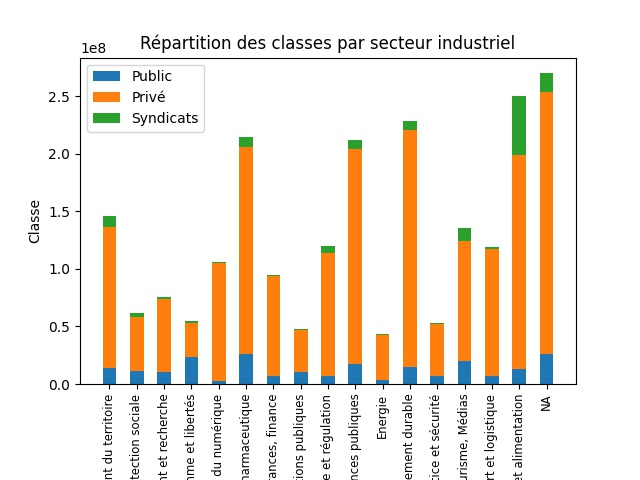
\includegraphics[scale=1]{croise_secteur_classif}
\label{fig}\caption{}\
\end{center}
\end{figure}
 

\begin{table}[h]
\footnotesize
\centering
\label{tab:secteurs}
\caption{Correspondance thèmes, secteurs et domaines}
\begin{tabularx}{\textwidth}{|>{\RaggedRight}X|>{\RaggedRight}p{12cm}|}
\hline
\textbf{Thèmes} & \textbf{Secteurs et domaines} \\
\hline
Construction, logement, aménagement du territoire & Occupation des sols - Patrimoine - Développement des territoires - Bâtiments et travaux publics - Construction, logement, aménagement du territoire - Logement - Construction \\
\hline
Aide et protection sociale & Assurance chômage - Handicap - Droit du travail - Dialogue social - Famille - Emploi, solidarité \\
\hline
Enseignement et recherche & Recherche et innovation - Education - Education, enseignement, formation - Enseignement supérieur, recherche, innovation - Éducation, enseignement, formation - Enseignement supérieur - Formation professionnelle - Statistiques \\
\hline
Droits de l'homme et libertés & Aide au développement - Humanitaire - Principe de précaution - Egalité femmes/hommes - Bien-être animal - Egalité des chances - Asile - Immigration - Discriminations - Questions migratoires - Société - Droits et libertés fondamentales - Liberté d’expression et d’information - Droits des victimes - Laïcité \\
\hline
Industries de télécommunications et du numérique & Accès à l’Internet - Accès aux moyens de télécommunications - Marché du numérique - Protection des données - E-commerce - Numérique - Télécommunications - Infrastructures de télécommunications - Marché du numérique - E-commerce \\
\hline
Santé et pharmaceutique & Médicaments - Remboursements - Soins et maladies - Système de santé et médico-social - Prévention - Santé - Système de santé et médico-social - Soins et maladies \\
\hline
Banques, assurances, finance & Banques, assurances, secteur financier - Protection des marques - Assurances - Finances - Banques - Banques, assurances, secteur financier et extra financier - Finances - Banques - Assurances \\
\hline
Gouvernance et institutions publiques & Outre-mer - Français de l’étranger - Collectivités territoriales - Pouvoirs publics et institutions - Institutions européennes - Institutions des outre-mer - Ordre administratif - Moralisation/Transparence - Coopération internationale - Accords internationaux - Economie des outre-mer - Développement économique des outre-mer \\
\hline
Concurrence et régulation & Secret des affaires / Secret professionnel - Aides aux entreprises - Brevet - Droit de la concurrence - Marchés réglementés - PME/TPE - Normes de production - Professions réglementées - Entreprises et professions libérales - Concurrence, consommation - Gouvernance d’entreprise - Commerce extérieur \\
\hline
Economie et finances publiques & Taxes - Politique industrielle - Fonction publique - Retraites - Partenariats public/privé - Finances publiques - Economie - Budget - Taxation - Impôts \\
\hline
Energies non-renouvelables & Energie nucléaire - Energie - Ressources naturelles - Ressources minières - Energies fossiles \\
\hline
Environnement et développement durable & Chasse - Eaux - Qualité de l'eau - Produits chimiques - Accidents et catastrophes naturelles - Impact des transports individuels - Impact des transports marchands et collectifs - Qualité de l'eau - Environnement - Déchets - Energies renouvelables - Impact de l'activité industrielle - Dépollution - Forêt - Occupation des sols \\
\hline
Justice et sécurité & Institutions judiciaires - Défense - Institutions pénitentiaires - Justice - Institutions judiciaires - Justice civile - Justice pénale - Défense, sécurité - Sécurité nationale - Sécurité routière - Espionnage et surveillance \\
\hline
Culture, loisirs, tourisme, Médias & Médias - Tourisme/hôtellerie - Droit d'auteur - Publicité - Musique - Sports - Propriété intellectuelle - Sports, loisirs, tourisme - Accès à la culture - Arts, culture - Musique - Spectacle vivant - Cinéma - Presse écrite - Audiovisuel - Jeux d'argent - Jeux-vidéo - Livre \\
\hline
Transport et logistique & Industrie aérospatiale - Services postaux - Infrastructures - Industrie aéronautique - Aéronautique, aérospatiale - Transports, logistique - Transport de voyageurs - Transport de fret - Transports alternatifs - Services postaux \\
\hline
Agriculture et alimentation & Sécurité et normes alimentaires - Appellations - Agriculture, agroalimentaire - Agriculture - Industrie agroalimentaire - Pêche \\
\hline\end{tabularx}
\end{table}
 

La encore, nous avons comparé plusieurs méthodologies pour effectuer cette classification, qui amènent à des répartitions proches et conforte la solidité de nos résultats. D'une part, chaque firme déclare des ``secteurs'' privilégiés. D'autre part, pour chaque action effectuée, une liste de ``domaines d'intervention'' est (parfois) indiquée. La première ambiguité est que la liste de tous les ``secteurs'' possibles n'est pas la m\^eme que celle de tous les ``domaines'' possibles, et ces deux listes sont de toute fa\c con trop grande pour une visualisation. Nous avons donc regroupé les domaines et secteurs du registre dans des grands thèmes, comme indiquée dans le tableau. La première méthodologie a été de comptabiliser les tiers suivant les thèmes des cabinets mandatés. La seconde méthodologie a été de les comptabiliser suivant les domaines des actions qui les concernent. Quand ces domaines ne sont pas indiqués, on peut choisir de prendre les 'secteurs' de la firme effectuant le lobbying, ou de simplement classifier l'action en 'NA'. Nous montrons les répartitions résultant des 4 scénarios, on présente également un tableau de corrélations, qui ne descendent pas en-dessous de 85\%.

\subsection{Responsables politiques visés}

Les firmes indiquent les décisions politiques concernées et les responsables politiques visés. Nous visualisons ici un croisement entre les catégories de responsables visés, et la classification des clients intéressés.


\begin{figure}[h!]
\begin{center}
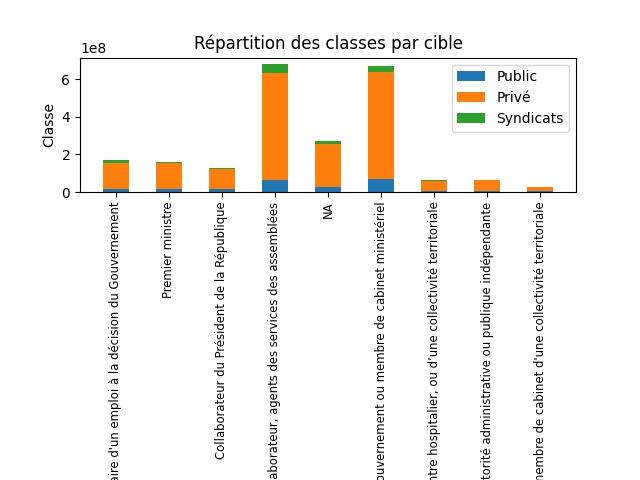
\includegraphics[scale=.5]{croise_cibles_classif}
\label{fig}\caption{}\
\end{center}
\end{figure}

  

\section{Problèmes des données et préconisations}


De manière générale, la qualité des entrées est insuffisamment contrôlée, comme en témoignent de nombreuses erreurs de saisie systématiques. 


En plus des limitations structurelles du fichier, les données comportent beaucoup de problèmes que nous évoquons à la section …,Les informations concernant les ressources financières et humaines des firmes de lobbying sont souvent absentes ou aberrantes (ce qui dénote en général une erreur de saisie). Nous pouvons montrer que les résultats sont robustes, car les pourcentages sont essentiellement conservées si l’on pondère le poids de chaque cabinet (et donc de ses clients) par les ressources financières et humaines que cette firme déclare allouer à la représentation d’intérêts. 

Une autre difficulté est que très peu d’informations sont obtenues sur les clients, en effet pour chaque action une liste de “tiers” pour laquelle l’action est menée est indiquée (et souvent absente), sans autre informations sur ces tiers. Nous avons été recherchés dans les données INSEE des informations supplémentaires sur ces tiers afin de les identifier dans la classification énoncée ci-dessus. Dans de nombreux cas, aucun tiers ni aucun client n’est indiqué, et l’action est imputée par défaut aux autres clients de ce cabinet, voire au cabinet en propre; nous avons pu montrer là aussi que les résultats sont robustes dans le sens où ils ne changent pas en fonction de la stratégie.


Commentaire sur l’empreinte normative?


Un second point important de cet article est d’évaluer statistiquement les failles des données présentes dans le répertoire. Un paradigme statistique est de définir une procédure automatique de détection de données erronées et de remplacement, et de comparer les résultats d’une étude transversale avec les données brutes et avec les données corrigées. Pour donner un exemple, les ressources brutes déclarées par secteur sont les suivantes [...] Si on applique désormais un algorithme de correction d’erreurs, elles sont les suivantes [...]. On observe que les résultats changent significativement pour l’agriculture, mais mois pour les autres (corrélation stat de 87\%). 

L’étude de l’influence présentée au 1er paragraphe est également robuste car les résultats après correction sont les suivants:...


\subsection{Détection des valeurs aberrantes}

\subsection{Préconisations sur les données}

Effectuons quelques recommandations simples sur la saisie des données qui permettront d'avoir accès à un panorama plus précis. 
Ces recommandations sont essentiellement techniques, mais d'autres recommandations structurelles ont été énoncées dans [Kerleo], qui permettraient encore une meilleure compréhension du lobbying. De manière évidente,  la granularité actuelle des budgets est trop vague, il serait bon d'indiquer la ventilation du budget annuel pour chaque action, et indiquer les contributions des tiers concernés au financement.
\begin{itemize}
\item Exiger plus d'informations sur les tiers; au minimum, les identifiants national type RNA et SIREN afin d'identifier chaque structure de manière non-ambigue et pouvoir récupérer leurs secteurs, objet social, ..., ou leurs pays d'affiliation pour les entitès étrangères.
\item Rendre cohérents la rubrique ``clients'' de la firme, avec les listes de ``tiers'' pour les actions déclarées. La pertinence d'avoir ces deux rubriques n'est pas claire.
\item Dans le m\^eme esprit, rendre cohérentes les ``secteurs'' déclarés sur la fiche d'une entreprise, et les ``domaines d'intervention'' qui accompagnent chaque action. Les listes de secteurs proposés dans ces deux catégories ne sont pas les m\^emes, et elles sont parfois contradictoires pour une firme donnée. Ici encore, on pourrait se contenter des domaines déclarés sur chaque action afin d'éviter de la redondance et de l'incohérence.
\item Appliquer des filtres statistiques simples de détections de valeurs aberrantes lors de la saisie, afin de demander des confirmations aux agents entrant ces données; et demander des budgets annuels exacts plut\^ot que des fourchettes.
\end{itemize}

  
 
   
\section{Conclusion}
Votre conclusion ici.

\% Bibliographie
\bibliographystyle{plainnat}
\bibliography{votre-bibliographie}

\end{document}
